% Chapter Template

\chapter{Ensayos y Resultados} % Main chapter title

\label{Chapter4} % Change X to a consecutive number; for referencing this chapter elsewhere, use \ref{ChapterX}

%----------------------------------------------------------------------------------------
%	SECTION 1
%----------------------------------------------------------------------------------------

Se realizaron pruebas funcionales sobre los requerimientos del proyecto.

\section{Ensayos preliminares sobre acerca del control de la plataforma mediante protocolo Firmata.}
\label{sec:Ensayos de control de la plataforma mediante protocolo Firmata}

Para comprobar el funcionamiento del entorno de depuración primero se comprobó mediante otro software el correcto acceso a la plataforma de hardware. Para esto se utilizó:

\begin{itemize}
	\item El programa \emph{Firmata test} \citep{firmataTest}, permite ensayar desde la PC el funcionamiento de una plataforma que soporte protocolo Firmata. La figura \ref{fig:firmataTest} expone la interfaz gráfica del software libre \emph{Firmata test}.
	\item La placa EDU-CIAA-NXP corriendo el programa Firmata4CIAA, el cual fue compilado y descargado de forma manual.
\end{itemize}

Se realizaron pruebas puntuales sobre los sensores y actuadores, demostrando el correcto acceso a todos los pines con sus respectivos modos de funcionamiento (los cuales pueden observarse en el Anexo I \ref{fig:MapeoPinesFirmata4CIAAv2}). 

\begin{figure}[!htbp]
	\centering
	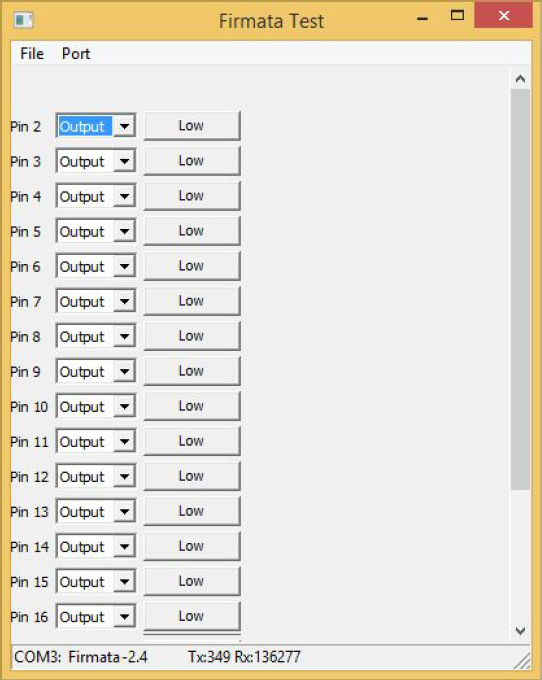
\includegraphics[width=12cm]{./Figures/firmataTest.png}
	\caption{Programa Firmata test}
	\label{fig:firmataTest}
\end{figure}

\begin{figure}[!htbp]
	\centering
	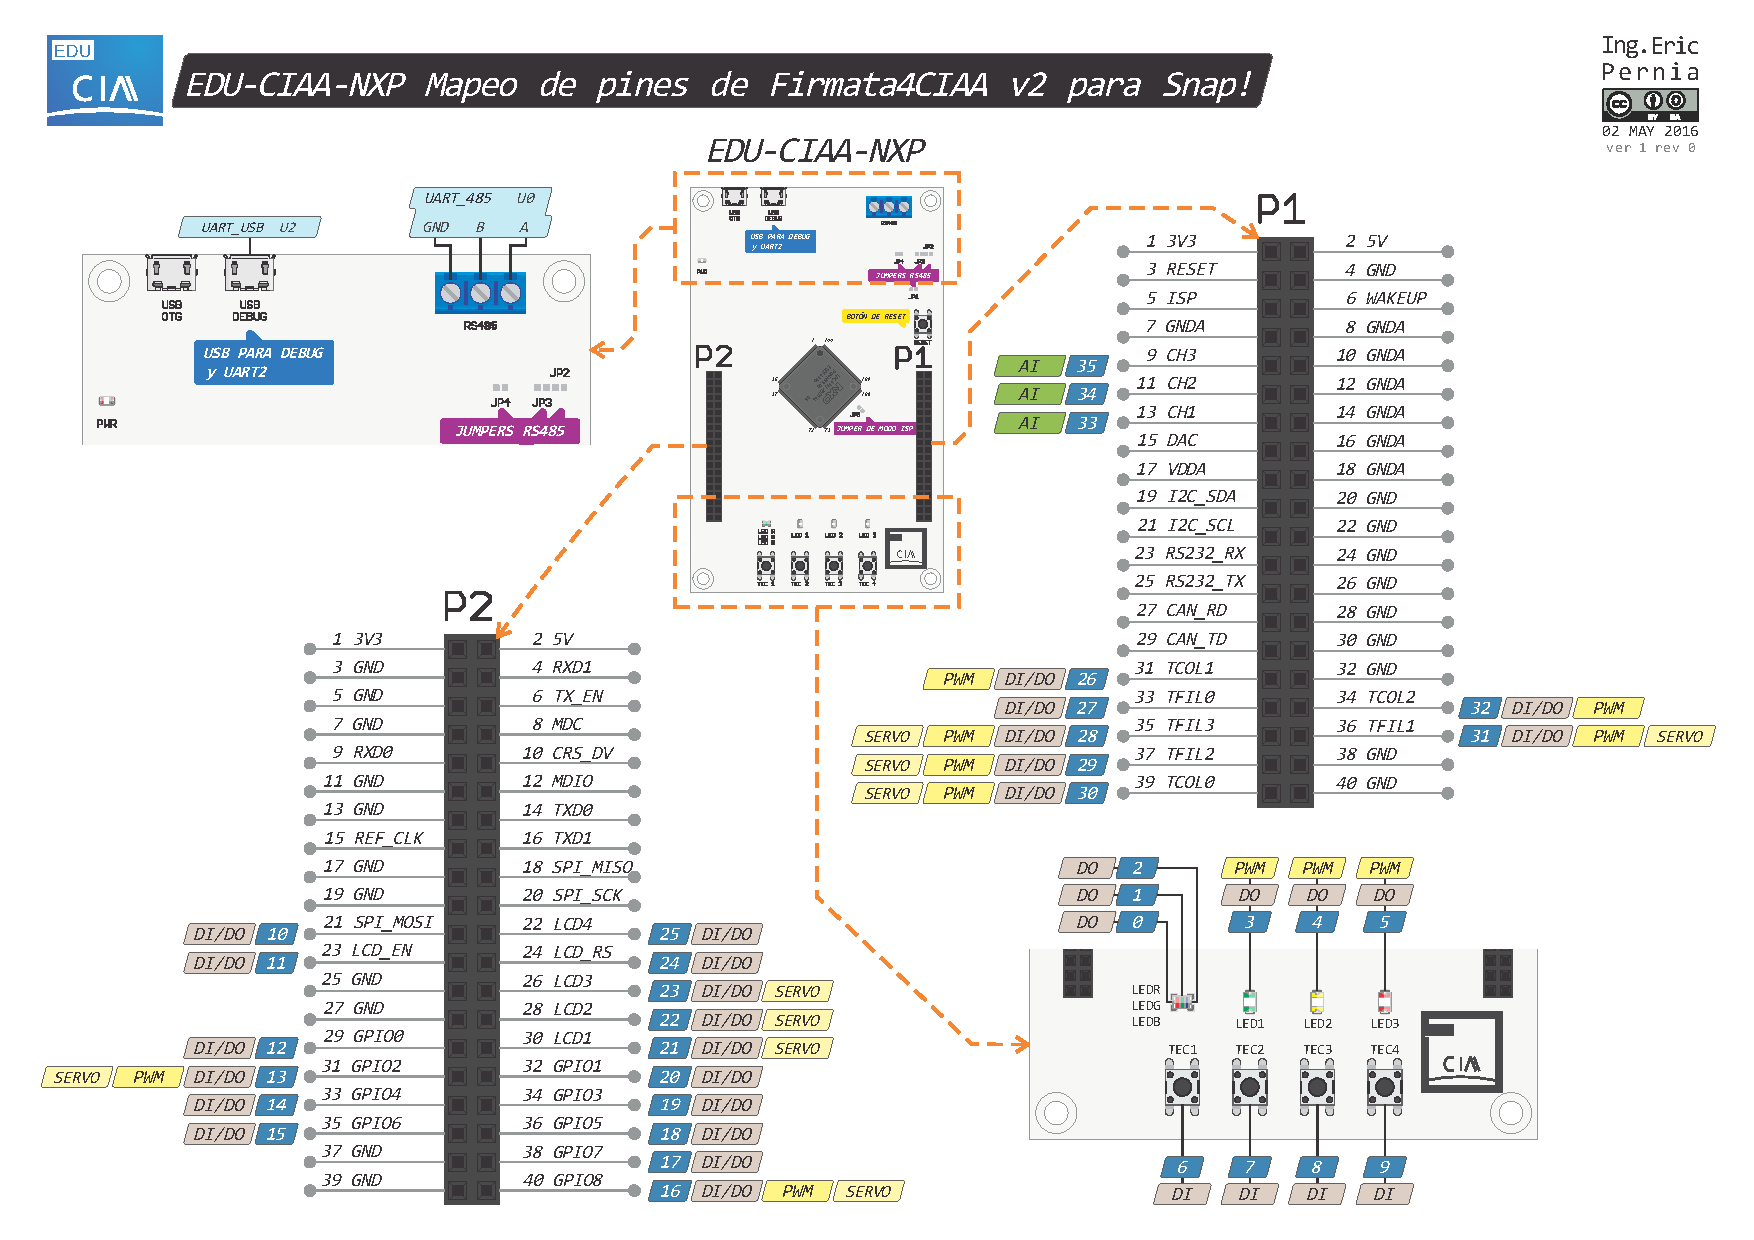
\includegraphics[width=12cm]{./Appendices/MapeoPinesFirmata4CIAAv2.pdf}
	\caption{Firmata4CIAA}
	\label{fig:MapeoPinesFirmata4CIAAv2}
\end{figure}

Para la verificación de Firmata de lado del cliente, se realizaron ensayos puntuales sobre la biblioteca \emph{Johnny five}. En la asignatura de Protocolos de Comunicación en Sistemas Embebidos de la CESE FIUBA \citep{CESE} se trabajo de forma puntual sobre el protocolo Firmata, realizando pruebas sobre un software web creado como trabajo final de la asignatura e instalado en la computadora, con el objetivo de ensayar todos los comandos del protocolo cliente sobre periféricos específicos conectados a la placa EDU-CIAA-NXP con Firmata4CIAA, y de esta manera realizar la manipulación de los mismos.  


\section{Ensayo de funcionamiento en los sistemas operativos Windows y Linux.}
\label{sec:Ensayo de funcionamiento en los sistemas operativos Windows y Linux.}

Este ensayo corresponde al “\emph{REQ1: El entorno de depuración deberá poder utilizarse dentro de los sistemas operativos Windows y Linux}”  y para llevarlo a cabo se realizaron los siguientes pruebas:

\subsection{Instalación en cada sistema.}
\label{subsec:Instalación en cada sistema.}

La instalación del sistema involucra la copia de los archivos necesarios para que el entorno de \emph{CIAABOT Debug} pueda funcionar sin problemas, en ambos sistemas operativos. 
Para llevar a cabo este \emph{test} se hizo la instalación en dos maquinas diferentes, una con el sistema operativo Windows y el otra con el sistema operativo Linux. 

El ensayo incluyó el proceso de descarga de los archivos del programa, y al ser exitosa, se ejecuto manualmente el siguiente \emph{test} funcional  sobre el estado \emph{Desconectado} para verificar de manera general el funcionamiento de \emph{CIAABOT Debug}. 

\subsubsection{\emph{Test} funcional posterior a la instalación en cada sistema}
Pre-condición:
\begin{itemize}
	\item \emph{CIAABOT Debug} se encuentra descargado en la computadora.
\end{itemize}
Flujo principal:
\begin{enumerate}
	\item
     Al Abrir \emph{CIAABOT Debug} se muestra al usuario la pantalla principal del entorno.
	\item
	El botón de inicio de sesión de depuración se muestra deshabilitado junto con las herramientas de control de ejecución.
	\item
	La edición de bloques del programa se encuentra habilitada.
\end{enumerate}

Resultado obtenido: en ambas computadoras se ejecutaron todos los pasos del \emph{test} sin problemas y de manera exitosa. 


\subsection{Chequeo de conexión y descarga de Firmata4CIAA.}
\label{subsec:Chequeo de acceso a puertos serie.}

Entre los archivos de \emph{CIAABOT Debug} se encuentra el archivo compilado que corresponde al proyecto de Firmata4CIAA  para la EDU-CIAA-NXP. Para proceder a la descarga de Firmata4CIAA, el entorno requiere que el usuario configure la ruta del \emph{toolchain} y de OpenOCD. Una vez realizado esto se comprobó mediante el siguiente \emph{test} manual la correcta comunicación entre el entorno, el \emph{toolchain} y \emph{openOCD}.

\subsubsection{\emph{Test} funcional descargar Firmata4CIAA}
Pre-condición:
\begin{itemize}
	\item
	\emph{CIAABOT Debug} se encuentra descargado en la computadora.
	\item
	La placa EDU-CIAA-NXP se encuentra conectada a la PC mediante el puerto marcado como \emph{USB Debug} en la serigrafía. La placa no tiene grabado el programa Firmata4CIAA.
\end{itemize}
Flujo principal:
\begin{enumerate}
	\item
	Al Abrir \emph{CIAABOT Debug} se muestra al usuario la pantalla principal del entorno.
	\item
    Al hacer click sobre el icono de configuración se muestra al usuario una ventana emergente para la configuración de los \emph{paths}.
	\item
	El usuario ingresa las rutas desde donde tiene el binario para el \emph{toolchain} y \emph{openOCD} y presiona el botón "Guardar".
	\item
	El usuario presiona el icono de actualizar desde la conexión con la plataforma.
	\item
	El entorno al estar en estado \emph{Conectado Sin Firmata4CIAA} consulta al usuario si quiere descargar Firmata4CIAA.
	\item
	El entorno avisa al usuario que la descarga fue exitosa.
\end{enumerate}

Resultado obtenido: en ambas computadoras se ejecutaron todos los pasos del \emph{test} sin problemas y de manera exitosa. 


\subsection{Chequeo de conexión con la plataforma EDU-CIAA-NXP.}
\label{subsec:Chequeo de conexión con la plataforma EDU-CIAA-NXP.}

El ensayo incluyó la comprobación del funcionamiento del inicio de la sesión de depuración para verificar que los bloques gráficos que acceden al hardware lo hagan de forma exitosa. Se ejecuto manualmente el siguiente \emph{test} funcional:

\subsubsection{\emph{Test} funcional de conexión con la plataforma EDU-CIAA-NXP}
Pre-condición:
\begin{itemize}
	\item
	\emph{CIAABOT Debug} se encuentra descargado en la computadora.
	\item
	La placa EDU-CIAA-NXP se encuentra conectada a la PC y con el programa Firmata4CIAA.
	\item
    El editor de programa de \emph{CIAABOT Debug} tiene importado un programa realizado en CIAABOT IDE.
\end{itemize}
Flujo principal:
\begin{enumerate}
	\item
	El programa de bloques se encuentra importado en el editor de programa de \emph{CIAABOT Debug}.
	\item
	Al usuario inicia la sesión de depuración haciendo click sobre el botón verde de \emph{debug}.
	\item
	El entorno habilita las herramientas de control de ejecución.
	\item
	El usuario hace click en el botón del icono \emph{ejecutar}.
	\item
	El entorno al detectar que existe un bloque gráfico con acceso a un periférico en particular, procede a realiza la conexión con la placa EDU-CIAA-NXP y muestra la manipulación del dispositivo al usuario.
\end{enumerate}

Resultado obtenido: en ambas computadoras se ejecutaron todos los pasos del \emph{test} sin problemas y de manera exitosa.



\section{Comprobación de funcionamiento de una sesión de depuración.}
\label{sec:Comprobación de funcionamiento de una sesión de depuración.}

Para poder verificar los siguientes requerimientos:

 \begin{itemize}
 	\item \emph{REQ2: Debe controlar de la ejecución de un programa corriendo en la plataforma de hardware}.
 	\item \emph{REQ3: Exponer el estado de las variables del programa en tiempo de ejecución}.
 \end{itemize}

 fueron necesarios realizar los siguientes ensayos de forma manual:

\subsection{Sesión de depuración uso del comando \emph{Ejecutar}}
Pre-condición:
\begin{itemize}
	\item \emph{CIAABOT Debug} se encuentra descargado en la PC.
	\item La placa EDU-CIAA-NXP se encuentra conectada a la PC y con el programa Firmata4CIAA.
	\item Existe un programa realizado en CIAABOT IDE con bloques gráficos de acceso al hardware.
\end{itemize}

Flujo principal:
\begin{enumerate}
	\item
	Al Abrir \emph{CIAABOT Debug} se muestra al usuario la pantalla principal del entorno. 
	\item
	El usuario elige el puerto serial desde donde tiene conectada la placa EDU-CIAA-NXP.
	\item
	El entorno detecta que la placa EDU-CIAA-NXP tiene descargado el programa Firmata4CIAA y habilita el inicio de sesión de depuración, mostrando el botón de \emph{debug} en color verde.
	\item
	El usuario presiona el botón verde de \emph{debug}.
	\item
	El entorno deshabilita la edición de programas, habilita las herramientas de control de ejecución y cambia el color del botón debug de verde a naranja.
	\item
	El usuario hace click en el botón de comando \emph{ejecutar}.
	\item
	El entorno ejecuta bloque por bloque el programa y al detectar que existe un bloque con acceso a un periférico envía la acción a la placa EDU-CIAA-NXP utilizando el protocolo firmata y muestra como salida la manipulación del dispositivo según lo programado por el usuario.
	\item
	El entorno actualiza el menú de visualización de variables con los nombres y valores de esas variables que se encuentran encastradas dentro de los bloques que están ejecutándose. 
\end{enumerate}

Resultado obtenido: ejecución de todos los pasos del \emph{test} en forma exitosa. 

\subsection{Sesión de depuración uso del comando \emph{Suspender}}
Pre-condición:
\begin{itemize}
	\item Sesión de depuración iniciada y programa en ejecución con el uso del comando \emph{ejecutar}.
\end{itemize}

Flujo principal:
\begin{enumerate}
	\item
	El entorno se encuentra ejecutando el programa con los bloques gráficos que acceden a periféricos como los que no acceden a periféricos.
	\item
	El usuario presiona el botón de \emph{suspender}.
	\item
	El entorno suspende la ejecución del programa, es decir, termina de ejecutar el bloque actual y se detiene antes del próximo bloque a ejecutar, el cual lo resalta con borde naranja.
	\item
	El usuario reanuda la ejecución del programa mediante el botón \emph{ejecutar}.
\end{enumerate}

Resultado obtenido: ejecución de todos los pasos del \emph{test} en forma exitosa.

\subsection{Sesión de depuración uso del comando \emph{Pasar por encima (step over)}}
Pre-condición:
\begin{itemize}
		\item Conexión con la plataforma establecida y la misma cuenta con Firmata4CIAA.
		\item Sesión de depuración iniciada. 
\end{itemize}

Flujo principal:
\begin{enumerate}
	\item
	El usuario hace click en el botón de comando \emph{Pasar por encima (step over)}.
	\item
	El entorno muestra resaltado el primer bloque del programa pero sin ejecutarlo.
	\item
	El usuario vuelve a hacer click en el botón de comando \emph{Pasar por encima (step over)}.
	\item
	El entorno muestra resaltado el bloque siguiente, ejecuta el bloque que fue resaltado anteriormente y actualiza el valor de las variables en el menú de visualizaciones de variables.
\end{enumerate}

Resultado obtenido: ejecución de todos los pasos del \emph{test} en forma exitosa.  

\subsection{Sesión de depuración uso del comando \emph{Pasar adentro (step into)}}
Pre-condición:
\begin{itemize}
	\item Conexión con la plataforma establecida y la misma cuenta con Firmata4CIAA.
	\item Sesión de depuración iniciada. 
\end{itemize}

Flujo principal:
\begin{enumerate}
	\item
	El usuario hace click en el botón de comando \emph{Pasar adentro (step into)}.
	\item
	El entorno muestra resaltado el primer bloque del programa pero sin ejecutarlo.
	\item
	El usuario vuelve a hacer click en el botón de comando \emph{Pasar adentro (step into)}.
	\item
	El entorno muestra resaltado el bloque siguiente, detecta que el bloque tiene un llamado a función y saltara a seleccionarlo. 
	\item
	El usuario vuelve a hacer click en el botón de comando \emph{Pasar adentro (step into)}.
	\item
	El entorno muestra resaltado el bloque siguiente dentro de la función y ejecutara el bloque anterior. 
\end{enumerate}

Resultado obtenido: ejecución de todos los pasos del \emph{test} en forma exitosa.  

\subsection{Sesión de depuración uso del comando \emph{Paso de regreso (step return)}}
Pre-condición:
\begin{itemize}
	\item Conexión con la plataforma establecida y la misma cuenta con Firmata4CIAA.
	\item Sesión de depuración iniciada y programa en ejecución con el uso del comando \emph{Pasar adentro (step into)}.
\end{itemize}

Flujo principal:
\begin{enumerate}
	\item
	El entorno se encuentra ejecutando el programa con los bloques gráficos resaltado los bloques con el uso del comando \emph{Pasar adentro (step into)} y ahora se encuentra dentro de una función.
	\item
	El usuario hace click en el botón de comando \emph{Paso de regreso (step return)}.
	\item
	El entorno ejecuta el bloque seleccionado y los siguientes sin seleccionarlos hasta encontrar el retorno de la función, luego seleccionara el siguiente bloque a continuación de la función que ejecuto.
\end{enumerate}

Resultado obtenido: ejecución de todos los pasos del \emph{test} en forma exitosa.  


\subsection{Sesión de depuración con puntos de ruptura (\emph{breakpoints})}
Pre-condición:
\begin{itemize}
     \item Sesión de depuración iniciada.
\end{itemize}

Flujo principal:
\begin{enumerate}
	\item
	El usuario hace \emph{click} con el botón derecho del \emph{mouse} en cualquiera de los bloques gráficos del programa.
	\item
	El entorno muestra el menú contextual del bloque desde donde se puede establecer el punto de interrupción.
	\item
	El usuario hace click dentro del menú contextual del bloque.
	\item
	El entorno establece el punto de interrupción en ese bloque, agrega un círculo rojo al mismo, en señal de \emph{breakpoint} y actualiza la ventana de visualización de puntos de ruptura con la información del nuevo \emph{breakpoint}.
	\item
	El usuario hace click en el botón del comando \emph{ejecutar}.
	\item
	El entorno ejecuta cada bloque de programa hasta llegar al bloque marcado con punto de interrupción donde detiene la ejecución y resalta el bloque con el \emph{breakpoint} que aún no ejecutó.
	\item
    El usuario hace click sobre el botón \emph{ejecutar}.
    \item
    El entorno continuará con la ejecución.
\end{enumerate}

Resultado obtenido: ejecución de todos los pasos del \emph{test} en forma exitosa. 


\subsection{Sesión de depuración uso del comando desactivar puntos de interrupción}
Pre-condición:
\begin{itemize}
	\item Sesión de depuración iniciada.
	\item Puntos de interrupción establecidos en algunos de los bloques.
\end{itemize}

Flujo principal:
\begin{enumerate}
	\item
	El usuario hace click en el botón de \emph{desactivar puntos de interrupción}.
	\item
	El entorno muestra el boton de \emph{desactivar puntos de interrupción} deshabilitado en señal de que se saltaran todos los puntos durante la ejecución  y actualiza el menú de visualización de puntos de ruptura (\emph{breakpoints}) mostrandolos desactivados.
	\item
	El usuario hace click en el botón del comando \emph{ejecutar}.
	\item
	El entorno resalta bloque por bloque el programa a medida que se va ejecutando sin detenerse al encontrar un punto de ruptura en el bloque establecidos anteriormente.
	\item
	El usuario hace click en el botón de \emph{desactivar puntos de interrupción}.
	\item
	El entorno muestra el botón de \emph{desactivar puntos de interrupción} habilitado y actualiza el menú de visualización de puntos de ruptura (\emph{breakpoints}) mostrandolos activados nuevamente.
\end{enumerate}

Resultado obtenido: ejecución de todos los pasos del \emph{test} en forma exitosa. 


\subsection{Sesión de depuración desactivar puntos de interrupción desde la ventana de visualización de \emph{breakpoints}}
Pre-condición:
\begin{itemize}
	\item Sesión de depuración iniciada.
	\item Puntos de interrupción establecidos en algunos de los bloques.
\end{itemize}

Flujo principal:
\begin{enumerate}
	\item
	El usuario hace click en uno de los \emph{checklist} actualmente tildado dentro del menú de visualización de puntos de ruptura (\emph{breakpoints}) de la columna “Activo”.
	\item
	El entorno muestra el \emph{checklist} destildado.
	\item
	El usuario hace click en el botón del comando \emph{ejecutar}.
	\item
	El entorno ejecuta los bloques de programa sin detenerse cuando encuentra el punto de ruptura en el bloque que fue destildado en la ventana de visualización de puntos de ruptura.
	\item
	El usuario hace click en el \emph{checklist} actualmente destildado dentro del menú de visualización de puntos de ruptura (\emph{breakpoints}) de la columna "Activo".
	\item
	El entorno ejecuta los bloques de programa y se detiene cuando encuentra el punto de ruptura en el bloque que fue tildado como activo desde la ventana de visualización de puntos de ruptura.
\end{enumerate}

Resultado obtenido: ejecución de todos los pasos del \emph{test} en forma exitosa. 


\subsection{Sesión de depuración uso del comando \emph{Detener depuración}}
Pre-condición:
\begin{itemize}
	\item Conexión con la plataforma establecida y la misma cuenta con firmata.
\end{itemize}

Flujo principal:
\begin{enumerate}
	\item
El entorno se encuentra con una sesión de depuración iniciada (se comprueban los casos con sesión en ejecución y con sesión de suspensión en ejecución).
	\item
	El usuario presiona el botón de \emph{detener depuración}.
	\item
	El entorno termina la ejecución del programa, finaliza la sesión de depuración, cambia el botón de \emph{debug} de color naranja a color verde y por ultimo habilita la edición del programa.
\end{enumerate}

Resultado obtenido: ejecución de todos los pasos del \emph{test} en forma exitosa. 

\subsection{Guardado y restauración de los puntos de ruptura}
Pre-condición:
\begin{itemize}
	\item \emph{CIAABOT Debug} se encuentra descargado en la PC.
    \item La placa EDU-CIAA-NXP se encuentra conectada a la PC y con el programa Firmata4CIAA.
    \item Existe un programa realizado en CIAABOT IDE y abierto en el editor de programas del entorno de \emph{debug}.
    \item Sesión de depuración iniciada.
\end{itemize}

Flujo principal:
\begin{enumerate}
    \item
	El usuario hace click derecho en cualquiera de los bloques gráficos que se muestran dentro del editor.
	\item
	El entorno muestra el menú contextual del bloque desde donde se puede establecer el punto de interrupción.
	\item
	El usuario hace click dentro del menú contextual del bloque.
	\item
	El entorno establece el punto de interrupción en ese bloque, agrega un punto rojo en señal de \emph{breakpoint} y actualiza la ventana de visualización de puntos de ruptura con la información del nuevo \emph{breakpoint}.
	\item
	El usuario hace click en el botón del comando \emph{ejecutar}.
	\item
	El entorno ejecuta los bloques de programa.
	\item
    El usuario detiene la sesión de depuración y cierra el programa, o abre otro programa.
	\item
	El entorno actualiza el archivo debug.cbd. dentro de la carpeta que contiene el proyecto automáticamente.
	\item
	El usuario hace click nuevamente en el menú "Proyecto" de la aplicación y abre el proyecto usado previamente  en el punto anterior.
	\item
	El entorno carga nuevamente el programa en el editor de \emph{debug}.
	\item
	El usuario comprueba que el punto de interrupción establecido anteriormente para ese bloque aparece nuevamente en el editor.
	
\end{enumerate}

Resultado obtenido: ejecución de todos los pasos del \emph{test} en forma exitosa. 


\section{Ensayos de edición de programas en lenguaje CIAABOT.}
\label{sec:Ensayos de edición de programas en lenguaje CIAABOT.}

Para poder verificar el requerimiento “\emph{REQ4: Permitir la edición de programas para corregir errores de lógica encontrados en tiempo de ejecución}”
fue necesario realizar el siguiente ensayo de forma manual:

\subsection{Edición de programa}
Pre-condición:
\begin{itemize}
	\item \emph{CIAABOT Debug} se encuentra descargado en la PC.
	\item La placa EDU-CIAA-NXP se encuentra conectada a la PC y con el programa Firmata4CIAA.
	\item Existe un programa realizado en CIAABOT IDE.
\end{itemize}

Flujo principal:
\begin{enumerate}
	\item
	Al Abrir \emph{CIAABOT Debug} se muestra al usuario la pantalla principal del entorno.
	\item
	El usuario elige el puerto serial desde donde tiene conectada la placa EDU-CIAA-NXP.
	\item
	El entorno detecta que la placa EDU-CIAA-NXP tiene descargado el programa Firmata4CIAA y habilita el inicio de sesión de depuración, mostrando el botón de \emph{debug} en color verde.
	\item
	El usuario realiza la modificación de los bloques gráficos, para ello agrega un nuevo bloque a la estructura de bloques del programa y guarda el programa actualizado desde el menú "Proyecto" de la aplicación.
	\item
	El entorno guarda el programa actualizado y actualiza el archivo .cbp dentro de la carpeta que contiene el proyecto guardado.
	\item
	El usuario hace click en el menú "Proyecto" de la aplicación y abre el proyecto que fue guardado en el punto anterior.
	\item
	El entorno carga nuevamente el programa en el editor de \emph{debug}.
	\item
	El usuario comprueba que el bloque gráfico agregado en el punto anterior se encuentre en el programa cargado.
\end{enumerate}

Resultado obtenido: ejecución de todos los pasos del \emph{test} en forma exitosa.


\section{Ensayos de interfaz de usuario.}
\label{sec:Ensayos de interfaz de usuario.}

Para poder verificar los requerimientos:
\begin{itemize}
	\item \emph{REQ5: La interfaz gráfica debe seguir los lineamientos de estilo establecidos en el Proyecto CIAABOT}.
	\item \emph{REQ6: Debe presentar un diseño de interfaz gráfica intuitiva, con elementos similares a los hallados en otras herramientas de depuración}.
\end{itemize}

Como parte de la verificación en los estilos visuales del diseño de la interfaz del entorno de \emph{debug} se realizaron reuniones con el director de este trabajo y con especialistas en diseño de interfaz de usuario para la evaluación de prototipos html, con la intención de descubrir errores en el funcionamiento que no cumplan los requerimientos, y ademas el de tener presente los posibles problemas de uso que podrían tener los usuarios.


\section{Validación con usuarios.}
\label{sec:Validación con usuarios.}

Para verificar el requerimiento “\emph{REQ6: Debe presentar un diseño de interfaz gráfica intuitiva, con elementos similares a los hallados en otras herramientas de depuración}” se realizaron ensayos de los usuarios finales en el marco de un laboratorio de programación llevado a cabo en la materia “\emph{Computadores 2 / Técnicas Avanzadas de Programación UNQ 2018}” \citep{computadores2unq2018} de la Universidad nacional de Quilmes. Los usuarios con experiencia de depuración en lenguaje C pudieron utilizar el entorno sin necesidad de algún soporte en la utilización de la herramienta de comandos para depuración que ofrece la plataforma, siendo esto prueba que el diseño de interfaz gráfica es intuitiva y de fácil uso.